

\chapter{Joint Executions}

\label{ch:jointexec}

This chapter constructs a new data structure for representing the
actions to be performed by a team of agents during the cooperative
execution of a shared task. Dubbed \emph{joint executions}, they are
partially-ordered branching sequences of actions that allow independent
actions to be performed independently, while using each agent's local
view to ensure that synchronisation is always possible when required.

The fundamental unit of reasoning in the situation calculus, and the
output of the standard Golog execution planning process, is the \emph{situation}:
a complete, ordered sequence of all actions that are to be performed.
This is suboptimal for representing plans in an asyncrhonous multi-agent
setting in three ways:

\begin{itemize}
\item it does not permit branching depending on information obtained at
run-time 
\item it enforces a strict execution order on actions that are potentially
independent, requiring inter-agent syncrhonisation when it is not
actually necessary 
\item it demands a strict execution order on actions that may be hidden
from some agents, demanding inter-agent synchronisation that is not
actually possible 
\end{itemize}
As we have demonstrated in Chapter \ref{ch:mindigolog}, restricting
the domain to be synchronous and completely known lets the agents
make effective use of raw situation terms for planning. But moving
to asynchronous domains with incomplete knowledge requires a more
powerful structure for representing the actions to be performed.

To build such a structure, we take inspiration from a model of concurrent
computation known as \emph{prime event} \emph{structures}, which are
partially-ordered branching sequences of events. A \emph{joint execution}
is defined as a particular kind of prime event structure that is rich
enough to capture the concurrent execution of independent actions,
and can branch on the sensing results of actions. It is also restricted
enough that it can be unambiguously reduced back to ordinary situation
terms for the purposes of reasoning. Using our explicit account of
the local \emph{view} of each agent from Chapter \ref{ch:observations},
we identify several restrictions on a joint execution that ensure
it is feasible to execute in the real world.

Joint executions thus allow us to capture the actions that a team
of agents are to perform in service of some shared task, without requiring
constant synchronization between the agents, and without assuming
that agents know all the actions that have been performed, while utilizing
existing reasoning methods based on ordinary situation terms. This
is a significant increase in expressiveness over existing approaches
to modeling multi-agent teams in the situation calculus. To demonstrate
the utility of the approach, we extend our MIndiGolog interpreter
from Chapter \ref{ch:mindigolog} to show how a team of agents can
cooperate to plan and perform the execution of a shared program in
an asynchronous, partially observable domain.

The chapter proceeds as follows: TODO.


\section{Background\label{sec:JointExec:Background}}

The above discussion highlighted three desirable properties of a plan
representation formalism intended for use in rich multi-agent domains:
it must be \emph{branching}, \emph{partially-ordered}, and \emph{feasible}.
While each of these aspects have been studied in isolation in the
situation calculus, our work is the first to combine them into a single
formalism suitable for a multi-agent setting.


\subsection{Branching}

Several single-agent formalisms based on the situation calculus have
introduced some form of branching into the structures returned by
the planner, including the conditional action trees of of sGolog \citep{lakemeyer99golog_cats}
and the branching IndiGolog plans of \citep{giacomo04sem_delib_indigolog}.
These structures typically branch based on the truth or falsehood
of test conditions included in the program, rather than directly on
the sensing results returned by an action. For example, the definition
of conditional action trees in \citep{lakemeyer99golog_cats} includes
the following branching case:\[
c=[\phi,c_{1},c_{2}]\]


This instructs the agent to execute the sub-tree $c_{1}$ if $\phi$
is true and the sub-tree $c_{2}$ if $\phi$ is false. While this
works well for a single agent, it is not clear how to extend it to
cooperative execution in a multi-agent setting, where some members
of the team may not know whether or not $\phi$ holds. Instead, we
will construct plans that branch directly on the results returned
by sensing actions, in the style of the {}``robot programs'' of
\citep{levesque96what_is_planning}.


\subsection{Partial Orders}

There has been little work on partial-order planning in the situation
calculus, most likely because the use of situations heavily biases
the reasoning machinery towards totally-ordered sequences of actions.
While \citet{son00htn_golog} allow the programmer to represent partial-orders
by adding operators to the Golog language, the actual plans produced
by their system are still raw situation terms. One exception is \citep{plaisted97sc_aspect},
which extends the situation calculus with explicit {}``aspects''
and allows partial ordering between actions that affect different
aspects of the world state. By contrast, we seek to leverage the existing
meta-theory of the standard situation calculus.

Partial-order planning is the mainstay of the closely-related event
calculus formalism. Here each action is specified to happen at a specific
time, and the constraints on relative occurrence times of actions
determine a partial ordering. \citet{Shanahan97ec_planning} has shown
that abductive theorem proving in the event calculate generates partially-ordered
plans, and the mechanics of the theorem prover naturally mirror various
concepts from partial-order planning literature, such as threats and
links \citep{peot92conditional_nonlinear}.

The close similarities between the situation and event calculi are
well understood, as are the advantages of the event calculus when
it comes to working with partially-ordered action sequences \citep{belleghem97sitcalc_evtcalc}.
Indeed, it is possible to implement a Golog interpreter on top of
the event calculus that naturally generates partially-ordered plans
\citep{pereira04ec_golog}. Perhaps we should simply adopt a formalism
such like the event calculus that is naturally partially-ordered,
rather than trying to construct partial orders on top of the naturally
sequential situation calculus?

While having a partial-order representation is important, it is not
the complete picture. We don't want the agents to have to synchronise
their actions unnecessarily, but we also need to ensure the converse:
that when an explicit ordering between actions is necessary, the required
synchronisation is actually possible. It is not clear how techniques
such as \citep{pereira04ec_golog} would extend to the asynchronous
multi-agent case.

As we shall see, the formalisms we develop in this thesis enable these
dual requirements - that some actions don't need to be ordered, while
other actions must not be ordered - to be captured in the situation
calculus in quite an elegant way.


\subsection{Feasibility}

To allow an agent to execute a plan that depends on information collected
at run-time, it is not sufficient to simply introduce branching into
the plan representation formalism. One must also ensure that, at execution
time, the agent will always \emph{know} which branch of the plan to
take. For example, suppose this simple branching plan will provably
achieve a goal:\[
\mathbf{if}\,\phi\,\mathbf{then}\, action_{1}\,\mathbf{else\,}\, action_{2}\]


The agent can only execute this program if it knows whether or not
$\phi$ holds; otherwise, although one of the branches is guaranteed
to achieve the goal, the agent does not know which one to take. Feasibility
is typically guaranteed by including sensing actions to ensure that
the test conditions are known:\[
sense_{\phi}\,;\,\mathbf{if}\,\phi\,\mathbf{then}\, action_{1}\,\mathbf{else\,}\, action_{2}\]


This requirement that an agent {}``knows how'' to execute a plan
is formalised by various notions of \emph{epistemic feasibility},
including those of \citep{levesque98what_robots_can_do,levesque00knowing_how,Lesperance01epi_feas_casl,giacomo04sem_delib_indigolog,baier06programs_that_sense}.

One approach to ensuring feasibility, embodied by \citep{levesque00knowing_how,giacomo04sem_delib_indigolog,baier06programs_that_sense},
is to represent plans by arbitrary programs formulated in a control
language such as Golog. One then semantically characterise the class
of epistemically feasible programs, using direct assertions about
the knowledge of each agent at each stage of execution. While this
allows for potentially very rich, very succinct plans, it is not clear
how to systematically generate an epistmically feasible plan from
such a general characterisation.

Another approach, advocated by \citep{levesque96what_is_planning,levesque98what_robots_can_do}
and used in the implementation section of \citep{giacomo04sem_delib_indigolog},
is to restrict the structure of plans so that they must be epistemically
feasible. For example, the {}``robot programs'' of \citep{levesque98what_robots_can_do}
are restricted to simple operators such as:\begin{gather*}
action\\
seq(\delta_{1},\delta_{2})\\
branch(action,\delta_{1},\delta_{2})\\
loop(branch(action,\delta,exit))\end{gather*}


These programs do not contain test conditions, but rather branch directly
on the (binary) sensing results returned from each action. There is
therefore no potential for confusion when executing such programs,
as they are essentially equivalent to a kind of finite automata that
can be executed reactively. Nevertheless, \citet{levesque98what_robots_can_do}
show that these programs are universal, in the sense that any achievable
goal can be achieved by suitable a robot program. We are not aware
of any work extending this approach to represent programs to be exeuted
cooperatively by a team of agents.

This notion of epistemic feasibility in a multi-agent setting can
be characterised as \emph{knowing what}. At each stage of execution,
each agent must know what its next action is. In synchronous domains
with public actions, as typically studied in the situation calculus,
this is sufficient to ensure the feasibility of executing a plan.

In asynchronous domains it is not enough for an agent to know \emph{what}
its next action is; it must also know \emph{when} that action should
be performed. For example, suppose that the following simple plan
provably achieves a goal:\[
action_{1}(agt_{1})\,;\, action_{2}(agt_{2})\]


In a synchrononous domain this plan can be executed directly. But
suppose the domain is asynchronous, and $agt_{2}$ is unable to observe
the occurrence of $action_{1}$. Since $agt_{2}$ has no way of knowing
whether or not $action_{1}$ has been performed, it will not know
when to perform $action_{2}$ and the plan cannot be executed.

In this chapter we adopt an approach similar to \citep{levesque98what_robots_can_do},
and define a restricted structure for representing plans that forces
all plans to be epistemically feasible. We use the explicit account
of each agent's local view developed in the previous chapter to ensure
that each agent will know when to perform its actions.


\subsection{Event Structures}

To tackle cooperative execution in a multi-agent setting, we have
adopted a model of concurrent computation known as \emph{event structures}
\citep{npw79event_structures}. The particular variant we are interested
in are \emph{prime event structures}, canonically defined as a four-tuple
as follows.

\begin{defnL}
[{Prime~Event~Structure}] A prime event structure is a four-tuple
$(\mathcal{V},\gamma,\prec,\oplus)$ where: $\mathcal{V}$ is a set
of events; $\gamma$ is a function assigning a\textbf{ }label to each
event; $\prec$ is the precedence relation, a strict partial order
on events; $\oplus$ is the conflict relation, a binary symmetric
relation indicating events that are mutually exclusive. 
\end{defnL}
The labels assigned by $\gamma$ represent the actions that may occur
in the world, and each event represents a potential occurrence of
an action. Which events can occur at each stage of execution is determined
by $\prec$ and $\#$. A \emph{configuration} is a sequence of events
consistent with $\prec$ in which no pair of events conflict. Each
configuration represents a potential partial run of execution of the
system.

As it can be cumbersome to specify $\prec$ and $\#$ in their entirety,
we will frequently give only the direct \emph{enablers} and \emph{alternatives}
for each event, denoted by $ens(i)$ and $alts(i)$ respectively.
Construction of $(\prec,\#)$ from $(ens,alts)$ is a straightforward
transitive closure. Formally, the enablers and alternatives of an
event are the largest sets satisfying:\begin{gather*}
j\in ens(i)\equiv j\prec i\,\wedge\,\forall k\in ens(i):\,\neg(j\prec k)\\
j\in alts(i)\equiv j\#i\,\wedge\,\forall k\in ens(i):\,\neg(j\#k)\end{gather*}


Considered in this way, event structures form a directed acyclic graph
of the events that could occur during execution of the system. As
shown in \citep{pratt91modeling_conc_with_geom}, these structures
are equivalent to a variety of formalisms for representing concurrent
execution (such as schedules and petri nets) and it is straightforward
to convert them into a kind of finite automaton for efficient execution,
much like the robot programs of \citep{levesque98what_robots_can_do}.


\section{Joint Executions\label{sec:JointExec:JEs}}

This section defines the precise structure of a joint execution, first
using a high-level intuitive description, and then formally as a set
of axioms to be included in the theory of action $\Dt$. Since we
intend for agents to synthesise joint executions as the output of
a planning process, they must exist as concrete terms in the logic.


\subsection{Intuitions}

We define a \emph{joint execution} as a special kind of prime event
structure as follows:

\begin{defnL}
[{Joint~Execution}] A joint execution is a tuple $(\mathcal{A},\mathcal{O},ens,alts,\gamma,<)$
where:\emph{ }action events $\mathcal{A}$ represent actions to be
performed; outcome\emph{ }events $\mathcal{O}$ represent possible
outcomes of actions; $(\mathcal{A}\cup\mathcal{O},ens,alts,\gamma)$
forms a prime event structure with precedence relation $\prec$; $<$
is a total order on events that is consistent with $\prec$.
\end{defnL}
It contains two disjoint sets of events: \emph{action} events $\mathcal{A}$
representing the actions to be performed, and \emph{outcome} events
$\mathcal{O}$ representing the possible outcomes of each action.
For each action event $i\in\mathcal{A}$, its enablers $ens(i)$ is
a set of outcome events, its alternatives $alts(i)$ is empty, and
its label $\gamma(i)$ is the action to be performed. For each outcome
event $i\in\mathcal{O}$, $ens(i)$ is a single action event for which
it is a possible outcome, $alts(i)$ is the set of all other outcome
events $j$ such that $ens(j)=ens(i)$, and $\gamma(i)$ is an outcome
as produced by the $Out(a,s)$ function for the action $\gamma(ens(i))$.

Each action event thus represent a single action to be performed,
which enables several alternate outcome events corresponding to the
potential results returned by that action. Each of these outcome events
can then enable further actions, and so forth.

A simple example of a joint execution is shown in Figure \ref{fig:example-je}.
Here action $act1$ has two possible outcomes, which enable different
actions $act2$ and $act3$. Recall that a \emph{configuration} is
a partial run of execution of the prime event structure. Clearly any
configuration ending in an outcome event corresponds to a unique history,
as it is a set of alternating actions and their outcomes.

%
\begin{figure}
\framebox{%
\begin{minipage}[t][1\totalheight]{1\columnwidth}%
\textsf{\textbf{\tiny 
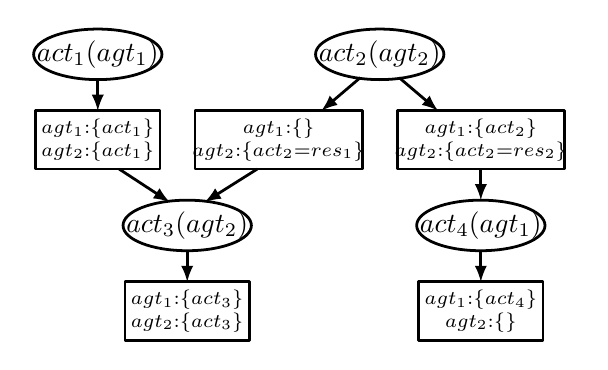
\begin{tikzpicture}[>=latex,join=bevel,scale=0.7]
  \pgfsetlinewidth{1bp}
%
\pgfsetcolor{black}
  % Edge: n1 -> n2
  \draw [->] (33bp,194bp) -- (33bp,178bp);
  % Edge: n3 -> n4
  \draw [->] (168bp,195bp) -- (148bp,178bp);
  % Edge: n3 -> n5
  \draw [->] (188bp,195bp) -- (208bp,178bp);
  % Edge: n6 -> n7
  \draw [->] (79bp,106bp) -- (79bp,90bp);
  % Edge: n8 -> n9
  \draw [->] (230bp,106bp) -- (230bp,90bp);
  % Edge: n2 -> n6
  \draw [->] (44bp,148bp) -- (70bp,131bp);
  % Edge: n4 -> n6
  \draw [->] (115bp,148bp) -- (88bp,131bp);
  % Edge: n5 -> n8
  \draw [->] (230bp,148bp) -- (230bp,132bp);
  % Node: n1
\begin{scope}
  \pgfsetstrokecolor{black}
  \draw (33bp,207bp) ellipse (33bp and 13bp);
  \draw (33bp,207bp) node {$act_1(agt_1)$};
\end{scope}
  % Node: n2
\begin{scope}
  \pgfsetstrokecolor{black}
  \draw (65bp,178bp) -- (1bp,178bp) -- (1bp,148bp) -- (65bp,148bp) -- cycle;
  \draw (33bp,163bp) node {$agt_1: \{act_1\} \atop agt_2: \{act_1\}$};
\end{scope}
  % Node: n3
\begin{scope}
  \pgfsetstrokecolor{black}
  \draw (178bp,207bp) ellipse (33bp and 13bp);
  \draw (178bp,207bp) node {$act_2(agt_2)$};
\end{scope}
  % Node: n4
\begin{scope}
  \pgfsetstrokecolor{black}
  \draw (169bp,178bp) -- (83bp,178bp) -- (83bp,148bp) -- (169bp,148bp) -- cycle;
  \draw (126bp,163bp) node {$agt_1: \{\} \atop agt_2: \{act_2=res_1\}$};
\end{scope}
  % Node: n5
\begin{scope}
  \pgfsetstrokecolor{black}
  \draw (273bp,178bp) -- (187bp,178bp) -- (187bp,148bp) -- (273bp,148bp) -- cycle;
  \draw (230bp,163bp) node {$agt_1: \{act_2\} \atop agt_2: \{act_2=res_2\}$};
\end{scope}
  % Node: n6
\begin{scope}
  \pgfsetstrokecolor{black}
  \draw (79bp,119bp) ellipse (33bp and 13bp);
  \draw (79bp,119bp) node {$act_3(agt_2)$};
\end{scope}
  % Node: n7
\begin{scope}
  \pgfsetstrokecolor{black}
  \draw (111bp,90bp) -- (47bp,90bp) -- (47bp,60bp) -- (111bp,60bp) -- cycle;
  \draw (79bp,75bp) node {$agt_1: \{act_3\} \atop agt_2: \{act_3\}$};
\end{scope}
  % Node: n8
\begin{scope}
  \pgfsetstrokecolor{black}
  \draw (230bp,119bp) ellipse (33bp and 13bp);
  \draw (230bp,119bp) node {$act_4(agt_1)$};
\end{scope}
  % Node: n9
\begin{scope}
  \pgfsetstrokecolor{black}
  \draw (262bp,90bp) -- (198bp,90bp) -- (198bp,60bp) -- (262bp,60bp) -- cycle;
  \draw (230bp,75bp) node {$agt_1: \{act_4\} \atop agt_2: \{\}$};
\end{scope}
%
\end{tikzpicture}

}}{\tiny {} }%
\end{minipage}}

\caption{ A simple joint execution. Elliptical nodes are action events, box
nodes are outcome events. }


\label{fig:example-je} 
\end{figure}


We will call a set of unordered, non-conflicting outcome events an
\emph{outcome set} and denote it $os$. A \emph{branch} is a special
case of an outcome set where every event is either in the branch,
conflicts with something in the branch, or precedes something in the
branch: \[
\forall i\in\mathcal{O}:\,\, i\in b\,\equiv\,\neg(\exists j\in b:\,\, i\oplus j\,\vee\, i\prec j)\]


A branch thus represents one potential \emph{terminating }run of execution.
TODO: demonstrate branches in the example JE.

The \emph{histories} of an outcome set, $hists(os)$, is the set of
all configurations that contain all elements of $os$, and end in
an event from $os$. By these definitions, the union of $hists(b)$
for all branches gives the set of all histories that could be produced
by performing the joint execution. 

A joint execution has one additional component over a standard prime
event structure: a \emph{total} order on events $<$ that is consistent
with the partial order $\prec$ induced by the enabling relation.
We will use this to perform reasoning by assuming that events occur
in the fixed order given by $<$, allowing them to be unambiguosly
translated into a \emph{canonical history}. When we come to use joint
executions for planning, we will restrict them so that every configuration
of the execution is equivalent to this canonical history. In practice,
$<$ would be determined by the order of insertion of events into
the structure.


\subsection{Formalities}

We introduce new sorts \noun{Event }and \noun{JointExec} to $\Lsit$,
and will collect the axioms defining joint executions in a separate
axiom set $\Dt_{je}$. Events are opaque identifiers with which a
joint execution associates a label, a set of enablers, and a set of
alternatives. For simplicity we will identify events with the integers,
although our definitions require only the successor function and ordering
relation. Labels are either \noun{Action} or \noun{Outcome} terms.


\subsubsection{Structural Axioms}

A joint execution consists of:

\begin{itemize}
\item a set of \emph{events}, which are integer ids
\item a mapping from each event to a \emph{label}, which is either an action
or an outcome
\item a mapping from each event to its \emph{enablers}, which is a set of
lower-numbered events
\item a mapping from each event to its \emph{alternatives}, which is a set
of events
\end{itemize}
As a base case, we have the empty joint execution as follows:

\[
JExec_{0}\,\isdef\, jexec(\{\},\{\},\{\},\{\})\]


The following four functions access the mappings contained in a joint
execution:\begin{gather*}
events(je)=es\,\equiv\exists ls,ns,as:\, je=jexec(es,ls,ns,as)\\
lblmap(je)=ls\,\equiv\exists es,ns,as:\, je=jexec(es,ls,ns,as)\\
ensmap(je)=ns\,\equiv\exists es,ls,as:\, je=jexec(es,ls,ns,as)\\
altsmap(je)=as\,\equiv\exists es,ls,ns:\, je=jexec(es,ls,ns,as)\end{gather*}


We also define the following shortcut accessors to get the value from
each mapping for a particular event $i$:\begin{gather*}
lbl(je,i,l)\equiv i\#l\in lblmap(je)\\
ens(je,i,ns)\equiv i\#ns\in ensmap(je)\\
alts(je,i,as)\equiv i\#as\in altsmap(je)\end{gather*}


For notational convenience we will often write these as functions,
but this should be understood as an abbreviation since not every joint
execution will contain every event. For example:\[
ens(je,i)=ns\,\isdef\,\exists ns':\, ens(je,i,ns')\wedge ns'=ns\]
Like standard situation terms, joint executions are built up by progressively
inserting new events into an existing joint execution. First, we have
a function to get the id of the next event:\[
NextEvent(je)=max(\{0\}\cup events(je))+1\]


To add to a joint execution, we must specify the predecessor joint
execution, the label for the new event, and its set of enablers. The
set of alternatives for the new event is determined automatically
based on the required structure of the joint execution -- action events
have no alternatives, while outcome events must have as their alternatives
every other outcome event enabled by the same action.

The following predicate specifies the conditions under which such
an insertion forms a valid joint execution, according to the intuitions
discussed above:\begin{gather*}
Insert(je,lb,ns,,je')\equiv\exists i:\, NextEvent(je)=i\\
\wedge\, events(je')=events(je)\cup\{i\}\\
\wedge\, lblmap(je')=lblmap(je)\cup\{i\#lb\}\\
\wedge\, ensmap(je')=ensmap(je)\cup\{i\#ns\}\\
\wedge\left(InsertOut(je,i,lb,ns,je')\vee InsertAct(je,i,lb,ns,je')\right)\end{gather*}


Note that this is not a function, since an invalid set of enablers
could cause it to be false. Outcome events must be enabled by a single
action event, and the alternatives must be updated for all other outcome
events associated with that action:\begin{gather*}
InsertOut(je,i,lb,ns,je')\equiv\,\,\,\,\,\, IsOutcome(lb)\\
\wedge\exists j,a:\, ns=\{j\}\wedge lbl(je,j,a)\wedge IsAction(a)\\
\wedge\left(\exists allAlts:\,\forall k:\, k\in allAlts\equiv ens(je',k,\{j\})\right)\\
\wedge\forall k:\,\left[k\not\in events(je')\,\rightarrow\,\neg\exists as:\, alts(je',k,as)\right]\\
\wedge\left[ens(je',k,\{j\})\rightarrow alts(je',k,allAlts)\right]\\
\wedge\left[\neg ens(je',k,\{j\})\rightarrow\exists as:\, alts(je,k,as)\wedge alts(je',k,as)\right]\end{gather*}


Action events must be enabled by a set of outcome events and cannot
have any alternatives:\begin{gather*}
InsertAct(je,i,lb,ns,je')\equiv\,\,\,\,\,\, IsAction(lb)\\
\wedge\forall j\in ns:\,\exists lb':\, lbl(je,j,lb')\wedge IsOutcome(lb')\\
\wedge altsmap(je')=altsmap(je)\cup\{i\#\{\}\}\end{gather*}


Finally, we need a second-order induction axiom stating that the only
joint executions are those that can be constructed in this way. This
is entirely analogous to the axiom for situation terms:\begin{multline*}
\forall P:\,\left[P(JExec_{0})\wedge\forall je,je',lb,ns:\, P(je)\wedge Insert(je,lb,ns,je')\rightarrow P(je')\right]\\
\rightarrow\forall je:\, P(je)\end{multline*}


These definitions enforece the basic structure of a joint execution,
but do not constrain it to be something that could be executed in
the world -- for example, outcomes can be enabled by actions that
will never actually produce that outcome. Like situation terms, we
focus first on getting the appropriate structure, and then specify
additional conditions that joint executions must satisify in order
to be legal in the real world.

Note that we have placed an important restriction on the ordering
of events -- if $i<j$ according to the total ordering over the integers,
then it is not possible for $i$ to be enabled by $j$. This does
not result in a lack of expressiveness, since if we want $i$ to be
enabled by $j$, then $j$ must not be enabled by $i$ and we can
simply give $j$ the lower event number.

Now, let us define the \emph{preceeds }and \emph{conflicts }relations
in terms of enablers and alternatives. We will write these as binary
infix operators $\prec_{je}$ and $\oplus_{je}$. The precedence relation
is defined as a transitive closure over enablers:\begin{multline*}
\forall P,i,j:\left[\left(i\in ens(je,j)\,\rightarrow P(i,j)\right)\,\wedge\,\left(\forall k:\, P(i,k)\wedge k\in ens(je,j)\,\rightarrow\, P(i,j)\right)\right]\\
\rightarrow\left(P(i,j)\rightarrow i\prec_{je}j\right)\end{multline*}


The conflict relation is defined so that $i\oplus j$ if they have
altnerative predecessors:\begin{multline*}
\forall P,i,j:\,\left[\left(i\in alts(je,j)\,\rightarrow P(i,j)\right)\right.\\
\left.\wedge\,\left(\forall i',j':\, P(i',j')\wedge i'\preceq_{je}i\wedge j'\preceq_{je}j\,\rightarrow\, P(i,j)\right)\right]\\
\rightarrow\left(P(i,j)\rightarrow i\oplus_{je}j\right)\end{multline*}


These axioms suffice to give an account of joint executions as prime
event structures as defined in \citep{npw79event_structures}.


\subsubsection{Additional Notions}

We also require some additional definitions and notation that is not
typically found in the literature on prime event structures, in order
to related joint executions back to the existing concepts of the situation
calculus.

An \emph{outcome set} is a set of unordered non-conflicting outcome
events; that is, a set of events satisfying:\begin{multline*}
OutSet(je,os)\,\equiv\,\forall i,j\in os:\, IsOutcome(lbl(je,i)\\
\wedge IsOutcome(lbl(je,j)\\
\wedge\,\neg(i\oplus_{je}j)\,\wedge\, i\not\prec_{je}j\,\wedge\, j\not\prec_{je}\, j\end{multline*}


An outcome set identifies a family of potential partial runs of the
execution. We can generate these histories by recursively selecting
an event that does not conflict with anything in $os$ and is enabled
given what we have performed so far:

TODO

An outcome set $os$\emph{ covers} a set \emph{$os'$,} denoted by
$os\sqsubseteq_{je}os'$, if every event in $os$ is either also in
$os'$, or precedes something in $os'$. Every history in $hists(os')$
will have a prefix in $hists(os)$. This defines a partial ordering
on outcome sets:\[
os\sqsubseteq_{je}os'\,\equiv\,\forall i\in os:\,\,\exists i'\in os':\,\, i\preceq_{je}i'\]


A \emph{branch}, denoted $b$, is a special case of an outcome set
that meets the following additional requirement:\[
Branch(je,b)\,\equiv\,\forall i\in events(je):\, i\in b\,\equiv\,\neg(\exists i'\in b:\,\, i\oplus i'\,\vee\, i\prec i')\]



\section{Independent Actions\label{sec:JointExec:IndepActs}}

As discussed in Section \ref{sec:Background}, posing queries in the
situation calculus requires a full situation term, which means a total
order on all actions that have occurred. The first step towards providing
only a \emph{partial} order on the actions to be performed is, therefore,
to capture the conditions under which actions can be performed out
of order without invalidating the results of the reasoning process.

Define \emph{independent} actions, identified by $indep(a_{1},a_{2},s)$,
as those that can be performed in either order, or even concurrently,
without affecting what holds in the resulting situation. Formally,
they must satisfy the following restrictions (where $\mathcal{P}$
and $\mathcal{F}$ are meta-variables ranging over predicate and functional
fluents respectively):

\begin{itemize}
\item $\mathcal{D}\,\models\, Poss(a_{1},s)\equiv Poss(a_{1},do(a_{2},s))$
and vice-versa 
\item $\mathcal{D}\,\models\, Out(a_{1},s)=Out(a_{1},do(a_{2},s))$ and
vice-versa
\item $\mathcal{D}\,\models\,\mathcal{P}(do(a_{1},do(a_{2},s)))\equiv\mathcal{P}(do(a_{2},do(a_{1},s)))$\\
 for all predicate fluents $\mathcal{P}(s)$
\item $\mathcal{D}\,\models\,\mathcal{F}(do(a_{1},do(a_{2},s)))=\mathcal{F}(do(a_{2},do(a_{1},s)))$\\
 for all functional fluents $\mathcal{F}(s)$
\end{itemize}
Whether actions are independent can be deduced from the description
of the action theory, or (as currently in our implementation) indicated
explicitly by the programmer.

We assume that the planning system has some way of identifying independent
actions. Two histories $\sigma_{1}$ and $\sigma_{2}$ are called
\emph{equivalent} if they are identical up to the ordering of independent
actions: they contain the same set of $(a,Out(a,s))$ pairs, and whenever
two such pairs occur in a different order in $\sigma_{1}$ than in
$\sigma_{2}$ the actions are independent. Two histories $\sigma_{1}$
and $\sigma_{2}$ are \emph{compatible for $a$ }if they are equivalent
after removing all actions that are independent of $a$. We then have
the following properties of histories:

\begin{thm}
\label{thm:equiv-holds}For equivalent histories $\sigma_{1}$ and
$\sigma_{2}$:\[
\mathcal{D}\,\models\,\mathbf{holds}[\phi,\sigma_{1}]\,\,\equiv\,\,\mathbf{holds}[\phi,\sigma_{2}]\]

\end{thm}
\begin{proof}
A straightforward case analysis on the definition of the regression
operator.
\end{proof}
\begin{thm}
\label{thm:equiv-legal}For equivalent histories $\sigma_{1}$ and
$\sigma_{2}$:\[
\mathcal{D}\,\models\,\mathbf{legal}[\sigma_{1}]\,\,\equiv\,\,\mathbf{legal}[\sigma_{2}]\]

\end{thm}
\begin{proof}
Using theorem \ref{thm:equiv-holds}, and invariance of $Poss$ and
$Out$ when transposing independent actions.
\end{proof}
\begin{thm}
\label{thm:equiv-compat}For histories $\sigma_{1}$ and $\sigma_{2}$
compatible for $a$:\begin{gather*}
\mathcal{D}\,\models\,\mathbf{holds}[Poss(a),\sigma_{1}]\,\,\equiv\,\,\mathbf{holds}[Poss(a),\sigma_{2}]\\
\mathcal{D}\,\models\,\mathbf{holds}[Out(a)=r,\sigma_{1}]\,\,\equiv\,\,\mathbf{holds}[Out(a)=r,\sigma_{2}]\end{gather*}

\end{thm}
\begin{proof}
Using Theorem \ref{thm:equiv-holds}, and the fact that the removed
actions do not affect the preconditions or outcome of $a$.
\end{proof}

\section{Legal Joint Executions\label{sec:JointExec:Legal}}

We now impose several restrictions on the structure of a joint execution,
to ensure they are suitable for representing the actions to be performed
by a team of agents. 

\textbf{(R1) Independent events have independent actions}\\
If the execution allows two action events to occur in either order,
then the corresponding actions must be independent. Formally, for
each $i_{1},i_{2}\in\mathcal{A}$:\[
i_{1}\prec i_{2}\,\vee\, i_{2}\prec i_{1}\,\vee\, i_{1}\#i_{2}\,\vee\, indep(\gamma(i_{1}),\gamma(i_{2}))\]


This restriction is key to the power of joint executions. It implies
that for every branch $b$, all histories in $hists(b)$ are equivalent.
By Theorem \ref{thm:equiv-holds} we can use the canonical history
for planning purposes, and be assured that the same fluents will hold
regardless of the specific order in which actions are executed. More
generally, it ensures that all histories in $hists(ens(i))$ are compatible
for $\gamma(i)$. By Theorem \ref{thm:equiv-compat} we can safely
use $hist(ens(i))$ to reason about the preconditions and outcomes
of $\gamma(i)$ using standard techniques.

\textbf{(R2) Every canonical branch history is legal}\\
For every branch $b$: \[
\mathcal{D}\,\models\,\mathbf{legal}[hist(b)]\]


By Theorem \ref{thm:equiv-legal} this ensures that every possible
run of execution of the system will produce a legal history.

\textbf{(R3) All possible outcomes are considered}\\
Planning clearly requires that all possible outcomes of an action
be considered. For each action event $i\in\mathcal{A}$, and each
possible outcome $r$ of that action, if:\[
\mathcal{D}\,\not\models\,\mathbf{holds}[Out(\gamma(i))\neq r,hist(ens(i))]\]


then there must be a corresponding outcome event:\[
\exists j\in E:\,\, ens(j)=\{i\}\,\wedge\,\gamma(j)=r\]


We can safely use the canonical history $hist(ens(i))$ to perform
this reasoning, thanks to R1.

\textbf{(R4) Actions are enabled by observable events:}\\
If an action event $i$ is enabled by an outcome event $j$ produced
by another agent, the agent performing $i$ must be able to observe
the occurrence of $j$. Otherwise, it has no way of synchronizing
its actions with those of its teammate. Let $actor(i)$ be the agent
responsible for performing an action event $i$, then we require that:\[
\forall j\in ens(i):\,\,\gamma(j)[actor(i)]\neq\{\}\]


If this restriction cannot be met, then the agents have no way of
synchronizing their actions. Construction of the joint execution must
therefore fail.

\textbf{(R5) Overlapping views enable identical actions:}\\
There must be no confusion about whether a particular action is enabled
at any point during execution. Lifting the function $view$ to operate
on sets of histories, then:\[
view(actor(i),\, hists(ens(i)))\]
 gives the set of all local histories after which $actor(i)$ is required
to perform the action $\gamma(i)$. Since the agent has only a local
viewpoint, it is possible that some other outcome set can produce
an identical view. Say that two outcome sets overlap, denoted $ovlaps(agt,e_{1},e_{2})$,
if they could produce an identical local history for a given agent:\[
view(agt,hists(e_{1}))\,\cap\, view(agt,hists(e_{2}))\,\neq\varnothing\]


Then the \emph{minimal overlapping set} for $e_{1}$, from the perspective
of $agt$, is the set of all $e_{2}$ satisfying:\begin{multline*}
e_{2}\in minovlp(agt,e_{1})\,\equiv\\
ovlaps(agt,e_{1},e_{2})\wedge\neg\exists e_{3}\left[ovlaps(agt,e_{1},e_{3})\wedge e_{3}\sqsubset e_{2}\right]\end{multline*}


This captures all outcome sets that the agent could potentially confuse
for $e_{1}$. To ensure there is no confusion about whether an action
is enabled, for each $i\in\mathcal{A}$, every $e$ in the minimal
overlapping set of $ens(i)$ for $actor(i)$ must enable an event
$i'$ with identical action $\gamma(i')=\gamma(a)$. Formally:\begin{multline*}
\forall e\in minovlp(actor(i),ens(i)):\,\\
\exists i':\,\gamma(i')=\gamma(i)\,\wedge\, ens(i')=e\end{multline*}
 This ensures that the agent's local information is enough to know
when it should perform an action. While it may not know precisely
which \emph{event} is enabled, it will know enough to determine the
specific \emph{action} that it must perform.%


\section{Planning with Joint Executions\label{sec:JointExec:Planning}}

Our implementation of an execution planning system uses joint executions
as an abstract data type that can be built up one event at a time,
one branch at a time. For a particular branch $b$, the state of the
world is reasoned about using standard regression techniques over
$hist(b)$, to determine the next action to perform. This action is
then be inserted into the joint execution to extend the branch.

Inserting a new action event requires specifying the action to be
performed, the branch on which to insert it, and a set of existing
events on that branch that must precede it. The code managing the
joint execution determines all possible outcomes of the action and
adds them as outcome events, returning a new branch for each outcome.
It also ensures that the restrictions in Section \ref{sub:Restrictions}
are satisfied, which can involve forcing an ordering between potentially
concurrent events to ensure independence (R1) or synchronization (R4),
or adding actions to other branches that the acting agent cannot distinguish
from the current one (R5). If the restrictions cannot be met, insertion
fails and the planner must backtrack to find a different action.

The intricacies of synchronization between agents in the face of partial
observability are thus hidden from the planning algorithm itself,
automatically managed by the construction of a joint execution.


\section{Summary\label{sec:JointExec:Summary}}

In this section we have defined a \emph{joint execution} as a prime
event structure with some additional restrictions. We contend that
such structures are highly suitable for planning the actions to be
performed by a team in service of some shared task, such as executing
a shared Golog program.

On one hand, joint executions are restricted enough to be practical
for such use. Prime event structures are purely reactive (equivalent
to a kind of finite automaton) and can be executed by the agents without
further deliberation. They are restricted to ensure that whenever
an agent is required to perform an action, it is able to determine
this using only its local information. Each branch of execution can
be easily converted into a situation term for the purposes of reasoning,
and can be extended one action at a time.

Joint executions are also significantly more flexible than previous
approaches. They allow independent actions to be performed without
synchronization, in any order. The agents need never know precisely
what actions have been executed, only those that enable them to perform
their next action. Synchronization is automatically achieved when
required by explicitly reasoning about what actions each agent can
observe, rather than requiring that all actions be public.

To demonstrate the utility of these structures, we have implemented
an interpreter for multi-agent ConGolog programs that produces joint
executions as its output. In the next section, we highlight the key
aspects of our implementation and give an example of the output it
produces.


\section{Implementation\label{sec:JointExec:Implementation}}

We have extended the implementation of a MIndiGolog execution planner
from Chapter \ref{ch:mindigolog} to utilise joint executions.

To make things more concrete, Figure \ref{fig:plan-output} shows
the output of our system when run on the $MakeSalad$ example of Figure
\ref{fig:makesalad-program}. Since all actions in this program have
a single outcome, the outcome events have been suppressed for brevity.

In this domain there are three agents, but only two chopping boards
are available. The agents must therefore synchronize their use of
these resources. Actions are taken to be independent if they deal
with different objects. As seen in Figure \ref{fig:plan-output},
the use of a partial order structure facilitates parallelism between
the agents, with each processing a different ingredient and only synchronizing
on the availability of the required resources. There is no need for
processing actions, such as $mix$ and $chop$, to be publicly observable.
This execution is maximally concurrent given the constraints of the
domain, and is clearly a significant improvement over totally ordered
sequences of actions as produced by existing systems.

In the following subsections, we briefly highlight some key aspects
of our implementation.


\subsection{Program Steps}

While the ability to determine whether actions are independent is
necessary in constructing partially-ordered executions of a ConGolog
program, it is not sufficient. Actions might have an order imposed
on them directly by the program (for example by the sequence construct
$a_{1};a_{2}$). The program may require that some additional conditions
are true immediately prior to executing an action (for example to
satisfy a test construct $\phi?$), which could be falsified by an
otherwise independent action.

To ensure that the dependencies between actions reflect the needs
of the program being executed, we augment our implementation of the
$Trans$ predicate to keep additional information about what transitions
were made. A \emph{step} object has the following attributes:

\begin{itemize}
\item action: the action performed in that step, or $nil$ if it is an internal
program transition 
\item test: an additional fluent formula that must hold immediately before
performing the step 
\item thread: a sequence of 'l' and 'r' characters indicating the concurrent
thread in which the step is performed 
\item outcome: the outcome of performing the action. 
\end{itemize}
%
\begin{figure}
\framebox{%
\begin{minipage}[t][1\totalheight]{1\columnwidth}%
\textsf{\textbf{\tiny 
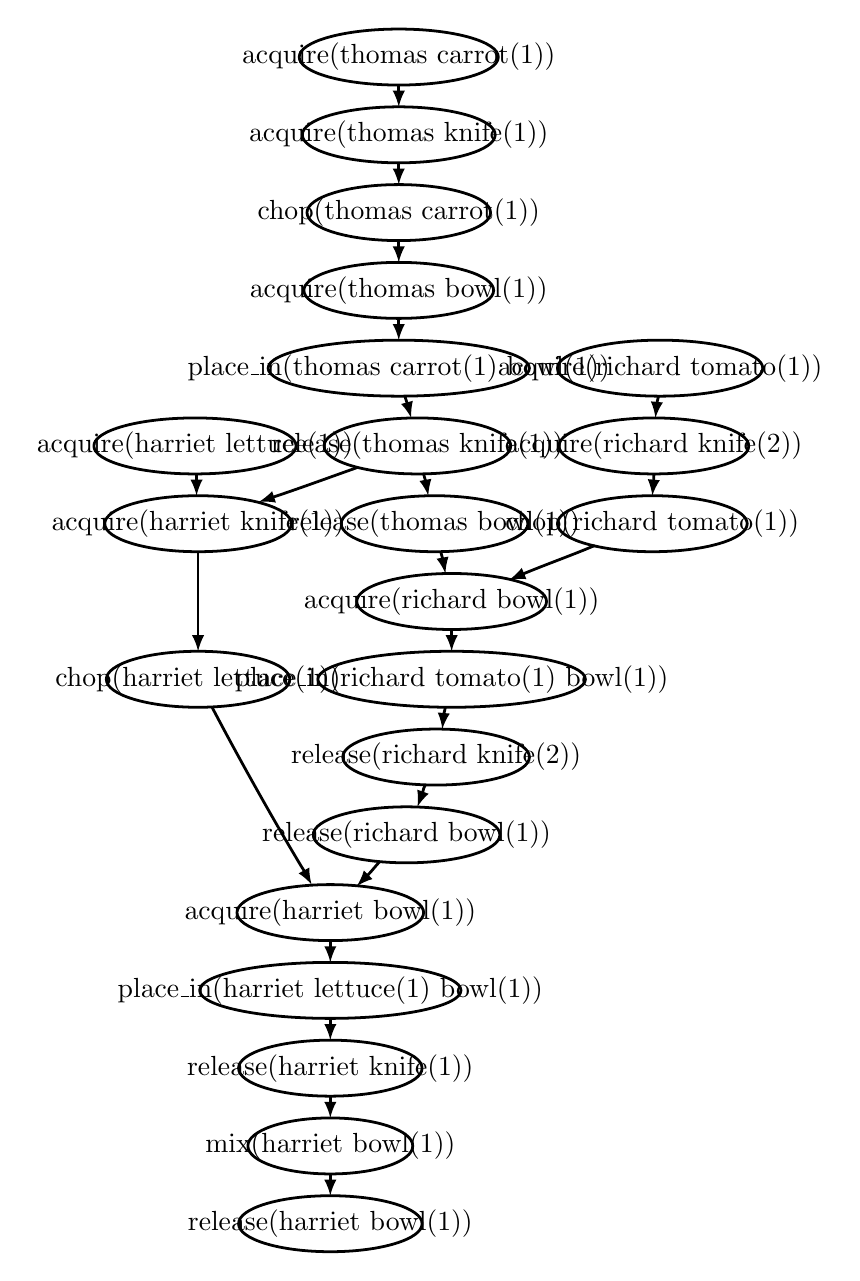
\begin{tikzpicture}[>=latex,join=bevel,scale=0.56]
  \pgfsetlinewidth{1bp}
%
\pgfsetcolor{black}
  % Edge: n0 -> n6
  \draw [->] (196bp,750bp) .. controls (196bp,749bp) and (196bp,748bp)  .. (196bp,736bp);
  % Edge: n2 -> n8
  \draw [->] (363bp,550bp) .. controls (363bp,549bp) and (362bp,547bp)  .. (361bp,536bp);
  % Edge: n6 -> n10
  \draw [->] (196bp,700bp) .. controls (196bp,699bp) and (196bp,698bp)  .. (196bp,686bp);
  % Edge: n8 -> n12
  \draw [->] (360bp,500bp) .. controls (360bp,499bp) and (360bp,497bp)  .. (359bp,486bp);
  % Edge: n10 -> n14
  \draw [->] (196bp,650bp) .. controls (196bp,649bp) and (196bp,648bp)  .. (196bp,636bp);
  % Edge: n14 -> n16
  \draw [->] (196bp,600bp) .. controls (196bp,599bp) and (196bp,598bp)  .. (196bp,586bp);
  % Edge: n16 -> n18
  \draw [->] (200bp,550bp) .. controls (200bp,549bp) and (201bp,547bp)  .. (204bp,536bp);
  % Edge: n18 -> n20
  \draw [->] (212bp,500bp) .. controls (212bp,499bp) and (213bp,497bp)  .. (215bp,486bp);
  % Edge: n18 -> n22
  \draw [->] (169bp,504bp) .. controls (152bp,498bp) and (133bp,491bp)  .. (106bp,482bp);
  % Edge: n4 -> n22
  \draw [->] (66bp,500bp) .. controls (66bp,499bp) and (66bp,498bp)  .. (66bp,486bp);
  % Edge: n20 -> n24
  \draw [->] (223bp,450bp) .. controls (223bp,449bp) and (224bp,447bp)  .. (226bp,436bp);
  % Edge: n12 -> n24
  \draw [->] (322bp,454bp) .. controls (308bp,448bp) and (291bp,442bp)  .. (267bp,432bp);
  % Edge: n22 -> n26
  \draw [->] (67bp,450bp) .. controls (67bp,435bp) and (67bp,413bp)  .. (67bp,386bp);
  % Edge: n24 -> n28
  \draw [->] (230bp,400bp) .. controls (230bp,399bp) and (230bp,398bp)  .. (230bp,386bp);
  % Edge: n28 -> n30
  \draw [->] (226bp,350bp) .. controls (226bp,349bp) and (225bp,347bp)  .. (224bp,336bp);
  % Edge: n30 -> n32
  \draw [->] (213bp,300bp) .. controls (212bp,299bp) and (212bp,297bp)  .. (208bp,286bp);
  % Edge: n32 -> n34
  \draw [->] (184bp,251bp) .. controls (181bp,248bp) and (179bp,245bp)  .. (169bp,235bp);
  % Edge: n26 -> n34
  \draw [->] (76bp,350bp) .. controls (88bp,327bp) and (111bp,285bp)  .. (132bp,250bp) .. controls (133bp,248bp) and (134bp,247bp)  .. (140bp,236bp);
  % Edge: n34 -> n36
  \draw [->] (152bp,200bp) .. controls (152bp,199bp) and (152bp,198bp)  .. (152bp,186bp);
  % Edge: n36 -> n38
  \draw [->] (152bp,150bp) .. controls (152bp,149bp) and (152bp,148bp)  .. (152bp,136bp);
  % Edge: n38 -> n40
  \draw [->] (152bp,100bp) .. controls (152bp,99bp) and (152bp,98bp)  .. (152bp,86bp);
  % Edge: n40 -> n42
  \draw [->] (152bp,50bp) .. controls (152bp,49bp) and (152bp,48bp)  .. (152bp,36bp);
  % Node: n0
\begin{scope}
  \pgfsetstrokecolor{black}
  \draw (196bp,768bp) ellipse (64bp and 18bp);
  \draw (196bp,768bp) node {acquire(thomas carrot(1))};
\end{scope}
  % Node: n2
\begin{scope}
  \pgfsetstrokecolor{black}
  \draw (364bp,568bp) ellipse (66bp and 18bp);
  \draw (364bp,568bp) node {acquire(richard tomato(1))};
\end{scope}
  % Node: n4
\begin{scope}
  \pgfsetstrokecolor{black}
  \draw (65bp,518bp) ellipse (65bp and 18bp);
  \draw (65bp,518bp) node {acquire(harriet lettuce(1))};
\end{scope}
  % Node: n6
\begin{scope}
  \pgfsetstrokecolor{black}
  \draw (196bp,718bp) ellipse (62bp and 18bp);
  \draw (196bp,718bp) node {acquire(thomas knife(1))};
\end{scope}
  % Node: n8
\begin{scope}
  \pgfsetstrokecolor{black}
  \draw (360bp,518bp) ellipse (61bp and 18bp);
  \draw (360bp,518bp) node {acquire(richard knife(2))};
\end{scope}
  % Node: n10
\begin{scope}
  \pgfsetstrokecolor{black}
  \draw (196bp,668bp) ellipse (59bp and 18bp);
  \draw (196bp,668bp) node {chop(thomas carrot(1))};
\end{scope}
  % Node: n12
\begin{scope}
  \pgfsetstrokecolor{black}
  \draw (359bp,468bp) ellipse (61bp and 18bp);
  \draw (359bp,468bp) node {chop(richard tomato(1))};
\end{scope}
  % Node: n14
\begin{scope}
  \pgfsetstrokecolor{black}
  \draw (196bp,618bp) ellipse (61bp and 18bp);
  \draw (196bp,618bp) node {acquire(thomas bowl(1))};
\end{scope}
  % Node: n16
\begin{scope}
  \pgfsetstrokecolor{black}
  \draw (196bp,568bp) ellipse (84bp and 18bp);
  \draw (196bp,568bp) node {place\_in(thomas carrot(1) bowl(1))};
\end{scope}
  % Node: n18
\begin{scope}
  \pgfsetstrokecolor{black}
  \draw (208bp,518bp) ellipse (60bp and 18bp);
  \draw (208bp,518bp) node {release(thomas knife(1))};
\end{scope}
  % Node: n20
\begin{scope}
  \pgfsetstrokecolor{black}
  \draw (219bp,468bp) ellipse (60bp and 18bp);
  \draw (219bp,468bp) node {release(thomas bowl(1))};
\end{scope}
  % Node: n22
\begin{scope}
  \pgfsetstrokecolor{black}
  \draw (67bp,468bp) ellipse (60bp and 18bp);
  \draw (67bp,468bp) node {acquire(harriet knife(1))};
\end{scope}
  % Node: n24
\begin{scope}
  \pgfsetstrokecolor{black}
  \draw (230bp,418bp) ellipse (61bp and 18bp);
  \draw (230bp,418bp) node {acquire(richard bowl(1))};
\end{scope}
  % Node: n26
\begin{scope}
  \pgfsetstrokecolor{black}
  \draw (67bp,368bp) ellipse (59bp and 18bp);
  \draw (67bp,368bp) node {chop(harriet lettuce(1))};
\end{scope}
  % Node: n28
\begin{scope}
  \pgfsetstrokecolor{black}
  \draw (230bp,368bp) ellipse (86bp and 18bp);
  \draw (230bp,368bp) node {place\_in(richard tomato(1) bowl(1))};
\end{scope}
  % Node: n30
\begin{scope}
  \pgfsetstrokecolor{black}
  \draw (220bp,318bp) ellipse (60bp and 18bp);
  \draw (220bp,318bp) node {release(richard knife(2))};
\end{scope}
  % Node: n32
\begin{scope}
  \pgfsetstrokecolor{black}
  \draw (201bp,268bp) ellipse (60bp and 18bp);
  \draw (201bp,268bp) node {release(richard bowl(1))};
\end{scope}
  % Node: n34
\begin{scope}
  \pgfsetstrokecolor{black}
  \draw (152bp,218bp) ellipse (60bp and 18bp);
  \draw (152bp,218bp) node {acquire(harriet bowl(1))};
\end{scope}
  % Node: n36
\begin{scope}
  \pgfsetstrokecolor{black}
  \draw (152bp,168bp) ellipse (84bp and 18bp);
  \draw (152bp,168bp) node {place\_in(harriet lettuce(1) bowl(1))};
\end{scope}
  % Node: n38
\begin{scope}
  \pgfsetstrokecolor{black}
  \draw (152bp,118bp) ellipse (59bp and 18bp);
  \draw (152bp,118bp) node {release(harriet knife(1))};
\end{scope}
  % Node: n40
\begin{scope}
  \pgfsetstrokecolor{black}
  \draw (152bp,68bp) ellipse (53bp and 18bp);
  \draw (152bp,68bp) node {mix(harriet bowl(1))};
\end{scope}
  % Node: n42
\begin{scope}
  \pgfsetstrokecolor{black}
  \draw (152bp,18bp) ellipse (59bp and 18bp);
  \draw (152bp,18bp) node {release(harriet bowl(1))};
\end{scope}
%
\end{tikzpicture}

}}%
\end{minipage}}

\caption{ Joint execution for $MakeSalad(bowl(1))$, showing significant concurrency
between agents }


\label{fig:plan-output} 
\end{figure}


We call a sequence of such steps a \emph{run}, which can be converted
to a history by taking just the action and outcome attributes. The
procedure implementing $Trans$ takes a program and a run as input,
returning a new program and new step of execution. As an example consider
the code in Figure \ref{fig:trans-code}, implementing the test operator
and the concurrency operator from equation \ref{eqn:trans_conc_orig}.

%
\begin{figure}
\framebox{%
\begin{minipage}[t][1\totalheight]{1\columnwidth}%
{\scriptsize \verbatiminput{listings/jointexec/ConGolog.oz}}%
\end{minipage}}

\caption{ Partial code for $Trans$ predicate }


\label{fig:trans-code} 
\end{figure}


Note that whenever the procedure descends through the left side of
a concurrency operator it pushes an 'l' onto the step's {}``thread''
attribute, and each descent through the right side pushes an 'r'.
Two steps can be said to come from different threads as long as neither
{}``thread'' attribute is a prefix of the other.

We say that two steps are \emph{ordered} if any of the following holds:
their action terms are not independent; ones thread is a prefix of
the other; ones action falsifies the test condition associated with
the other. When building a joint execution, ordered steps are forced
to be executed in the order they were generated by the planner, while
unordered steps may be performed independently.


\subsection{Planning Procedure}

The code for planning a joint execution from a given ConGolog program
is shown in Figure \ref{fig:planning-code}. The main procedure is
$MakePlan$, a recursive procedure that operates on a list of branches-in-progress
of the form $(D,R,B)$. Here $B$ is a branch in the joint execution
under construction, $D$ is the program remaining to be executed on
that branch, and $R$ is the run of program steps performed on that
branch so far.

%
\begin{figure}
\framebox{%
\begin{minipage}[t][1\totalheight]{1\columnwidth}%
{\scriptsize \verbatiminput{listings/jointexec/Planner.oz}}%
\end{minipage}}

\caption{ Code for main planning loop }


\label{fig:planning-code} 
\end{figure}


%
\begin{figure}
\framebox{%
\begin{minipage}[t][1\totalheight]{1\columnwidth}%
{\scriptsize \verbatiminput{listings/jointexec/psearch.oz}}%
\end{minipage}}

\caption{ Code to run planning procedure in parallel }


\label{fig:parallel-search} 
\end{figure}


Each iteration of the planning loop proceeds as follows. The procedure
$FindOpenBranch$ updates each branch to account for events that were
added since it was last processed (some may have been added automatically
to satisfy restriction (R5)), then searches the list to find a branch
for which $Final(D,R)$ does not hold. If all branches are final,
planning can terminate. Otherwise, the procedure $FindTrans1$ is
called to find a new step of execution for that branch. The action
is inserted into the joint execution, which returns a list of new
branches, one for each possible outcome of the action. Each of these
outcomes is added to the list of branches, and the loop is started
again.

Of particular interest is the procedure $FindTrans1$, which uses
the encapsulated search functionality of Mozart to yield possible
next steps according to an estimate of their potential for concurrency.
The procedure $LP.yieldOrdered$ yields the solutions of the given
search context, sorted using the procedure $CompareSteps$. This procedure
(not shown) gives preference to steps that can be performed concurrently
with as many existing actions as possible.


\subsection{Distributing the Planning Workload}

A primary motivation in using Mozart/Oz for our implementation is
its strong support for distributed logic programming. Utilizing Mozart's
parallel search functionality \citep{Schulte00constraint_services},
the planning workload can be transparently distributed between the
agents in the team.

Figure \ref{fig:parallel-search} shows the necessary code, which
should be executed by one of the agents. The planning procedure is
encapsulated in a \emph{functor}, a portable code object. A parallel
search object is then created, which uses an ssh connection to spawn
remote computations on each of the three agents (identified by their
DNS names). The object is asked to provide a single solution, which
is then written to a file in the graphviz 'dot' format for display
(resulting in Figure \ref{fig:plan-output}).

For the simple example shown in this chapter, parallel plan search
does not demonstrate a significant time saving since almost no backtracking
is required to reach a solution. For more difficult problems, significant
gains can be expected.


\section{Discussion\label{sec:JointExec:Discussion}}

An alternate approach to the problem of partial observability is the
language TeamGolog developed in \citep{farinelli07team_golog}, where
agents explicitly synchronize through communication and a shared state.
By contrast, our approach constructs synchronization implicitly by
reasoning about the actions that can be observed by each agent. This
has the advantage of requiring no changes to the form or semantics
of the agents' control program, but the disadvantage that joint execution
construction may fail if too many actions are unobservable. It would
be interesting to combine these approaches by automatically incorporating
explicit communication when implicit synchronization is not possible.

There is, of course, an extensive body of work on partial-order planning
in the context of goal-based planning. Unsurprisingly, the joint execution
structure we develop here has deep similarities to the structures
used in conditional partial-order planners such as \citep{peot92conditional_nonlinear}.
It is, however, intentionally specific to the situation calculus.
We make no use of many concepts common in partial-order goal-based
planning (causal links, threats, conflicts, etc) because we do not
deal explicitly with goals, but with steps generated by an underlying
transition semantics. Our approach can be considered roughly equivalent
to \emph{deordering} of a totally-ordered plan as described in \citep{backstrom99reordering},
except performed during plan construction rather than as a post-processing
step.



loops: \citep{levesque96what_is_planning,levesque05planning_with_loops}

